%---------- COURSE INFORMATION ------------------------
\newcommand{\course}{CIS 489-01}
\newcommand{\coursetitle}{CAPSTONE HCI/UX PROJECT}
\newcommand{\courseloc}{Keller 234}
\newcommand{\coursetime}{Monday 6 p.m. - 8:45 p.m.}
\newcommand{\coursedesc}{This interdisciplinary, collaborative course integrates theoretical concepts and practical skills gained in courses in the HCI/UX minors and associated majors into a capstone project. The course presents real-world problems through case studies and assignments that emphasize the student's communication, collaboration, technical, project management, design, and problem solving skills.}

\newcommand{\coursesec}{01}
\newcommand{\coursecredithours}{3}
\newcommand{\courseprereq}{None.}
\newcommand{\coursedelmethod}{Traditional Classroom}

\newcommand{\courseobjectives}{\item Explain interaction design techniques and the benefits of using interaction design principles for software development.
	\item Expand the concept of traditional usability to a broader notion of user experience.
	\item Experience hands-on, practical team-work engaging in the process of the iterative evaluation-centered UX lifecycle.
	\item Embrace design thinking and ideation to address the new characteristics embodied within user experience
	\item Describe and experience agile UX development methods.
	\item Work in a team environment on a project using interaction design creation and refinement activities such as:
		\begin{enumerate}
		\item Requirements extraction
		\item Design-informing modeling for conceptual and detailed design
		\item Establishing user experience goals, metrics and targets
		\item Building rapid prototypes
		\item Performing formative user experience evaluation
		\item Using iterative interaction design refinement
		\end{enumerate}
}

\newcommand{\coursetopics}{\item Usability of Interactive Systems
	\item Agile Design Methodology with Scrum
	\item Contextual Inquiry and Analysis
	\item Design Requirements (Needfinding)
	\item Design Thinking, Ideation, and Sketching
	\item Mental Models and Conceptual Designs
	\item HCI/UX Goals, Metrics, and Target
	\item Rapid Iterative Prototyping
}
\newcommand{\coursegrades}{Subject Exams (2 exams @ 20\% each)\dotfillsmall 40\% \\
		Project Work\dotfillsmall 30\% \\
		Final Project\dotfillsmall 30\% }
\newcommand{\coursetext}{
	\adjustbox{valign=c}{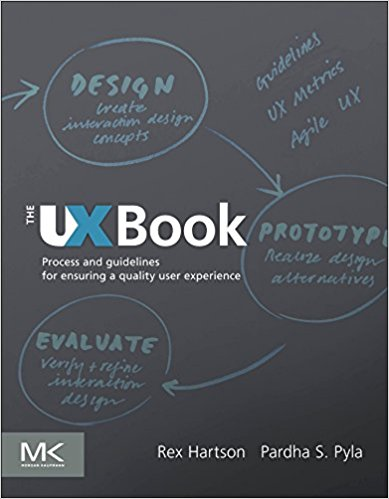
\includegraphics[width=1in]{img/cis489}} & \hangindent .4in \textbf{Textbook:} Hartson, R., Pyla, P., (2012)., he UX Book: Process and Guidelines for Ensuring a Quality User Experience (1st edition). Morgan Kaufmann. ISBN-10: 0123852412, ISBN-13: 978-0123852410. \\
	%& \hangindent .4in Simulation Software: SAM 365 \& 2016 Assessments, Trainings, and Projects with MindTap Reader.
}